\documentclass{article}

% For figures
\usepackage{graphicx} % more modern
\usepackage{subfigure} 

% For citations
\usepackage[round]{natbib}

% For algorithms
\usepackage{algorithm}
\usepackage{algorithmic}
\usepackage{hyperref}
\newcommand{\theHalgorithm}{\arabic{algorithm}}
\usepackage{mathtools}
\usepackage{amsmath}
\usepackage{kbordermatrix} %http://www.hss.caltech.edu/~kcb/TeX/kbordermatrix.sty

\usepackage{multicol}

\begin{document} 

\title{Garden Economy: Using ecological information metrics to shed light on economic vitality}
\author{Becky Roselius Haney}
\maketitle


\begin{abstract} 
Macroeconomic policy has an ill-defined optimization
problem: max Y. That is, guiding principle for nearly all
policy decisions is to maximize GDP - Gross Domestic Product. GDP
is equal to National Income, thus, striving to maximize GDP
is analogous to a business using maximum revenue as its guiding
principle. what would a well-defined macroeconomic optimization
problem look like? It would maximize something like ``well-being''
or ``economic vitality'' subject to binding constraints.~\footnote{Associate 
Professor of Economics, Calvin College, 1740 Knollcrest Cir SE, Grand Rapids, MI USA. This research
has been generously underwritten by a Calvin College 
sabbatical grant.}
\end{abstract} 

%\begin{multicols}{2}

\section{How does your garden grow?}

In 19xx, millions of the most productive hectares of wheat fields
in the ``bread basked of America'' turned
to dust, seemingly overnight. The top soil was churned up by 
fierce winds to create nightmarish dust storms that lasted
for nearly a decade. Bankrupt
farmers were forced to move. Those who chose to stay lived
in poverty or died from maladies associated with the incessant
storms of dust. While there are many causes cited for 
this dust bowl era, there is no doubt that it was a man-made
catastrophe. The prairie lands had thrived for
hundreds of years in the face of similar natural conditions  before settlement.
Drought tolerant buffalo grass, with its deep roots, served
as an anchor for the entire ecosystem. The ruthless forces of 
evolution had made sure of that. Any element of the ecosystem
that could not take the harsh winds and water-less seasons
did not last. And yet, this prairie, left mostly untouched
by human society, supported a thriving population of
flora and fauna. In XXXX, over XXXXX heads of buffalo
as well as.....prairie dogs, etc......survived and thrived
in those harsh conditions.

The ecosystem that existed before the settlers came was abundantly
resilient. It weathered extreme droughts and extreme rains well.
But, entrepreneurs and others who came across that
empty prairie in the late nineteenth century could be excused for 
looking at all those seemingly empty acres and thinking they were
going to waste.  Acres such as these, could be
more efficiently used to produce much needed food for the 
the burgeoning American population that was desperately
 in need of bread.
 



Through technology and back-breaking labor
these vacant acres of prairie were transformed
to highly efficient (from the human standpoint) food
production. Thus, settlers, risk-takers, and those without many other
good options, were enticed to move from the east to
what appeared to be empty land and stake a claim. Families
were given loans for farm equipment and seed. County
extensions cropped up to help explain best practices for farming.
From XXXX to XXXX over XXXX bushels of wheat were produced.
Indeed, the productivity proved almost too good. 
The acres were so productive
that the abundant supply dropped the price of wheat to
levels that wouldn't support the farms.  
The government then
provided price supports and farming continued.

However, the the prices bottoming-out were not the only
evidence that this economy had over-shot the 
optimal point of efficiency. As more land was added to arable
fields, land that had become less productive had to be
augmented with chemicals.
The land kept producing, but it also became vulnerable to 
weather extremes. 

When the extreme droughts of 19xx and 19xx hit, the highly efficient, 
productive economy
crashed unceremoniously. ... what happened?   ...

\begin{figure}
\centering\
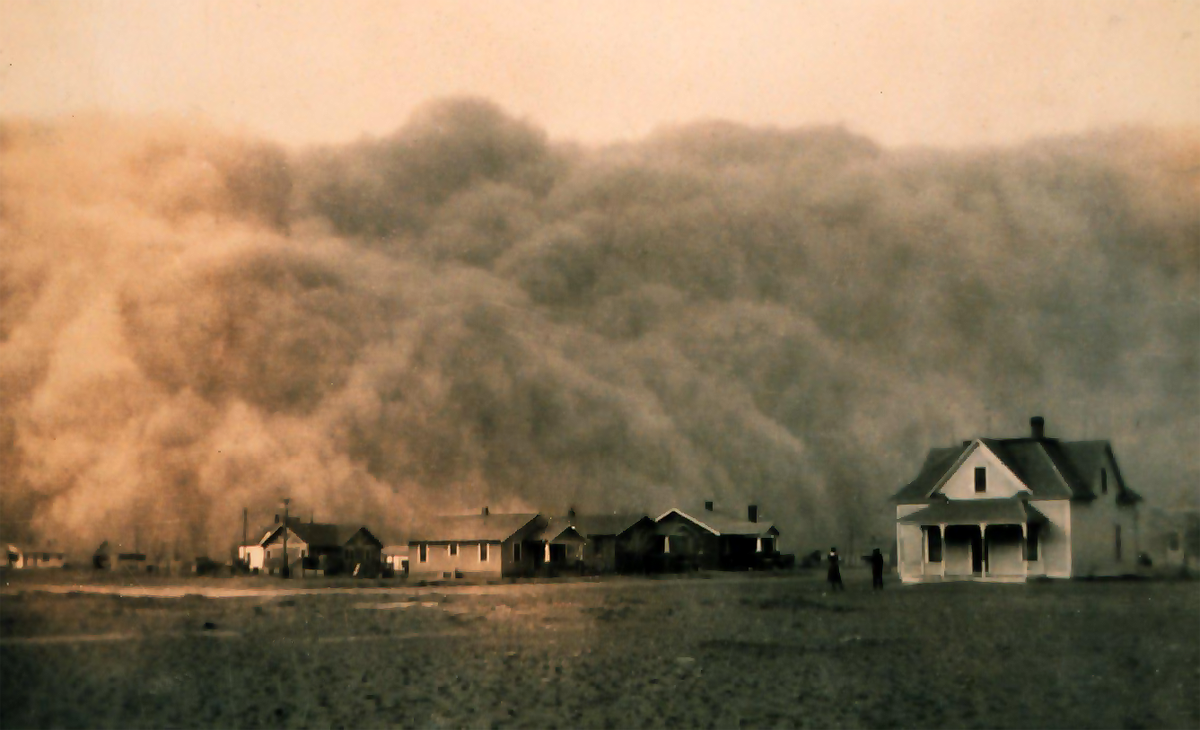
\includegraphics[width=.9\linewidth]{Dust-storm-Texas-1935.png}
\caption{``Black Blizzard'' Texas, 1935.}
\label{fig:ulano_ex}
\end{figure}

%{By Credit: NOAA George E. Marsh Album - Source: original upload 7 March 2005 in english wikipedia by w:en:User:Brian0918; there from %http://www.photolib.noaa.gov/htmls/theb1365.htmSource: original upload 7 March 2005 in english wikipedia by w:en:User:Brian0918; there from welding training, Public %Domain, https://commons.wikimedia.org/w/index.php?curid=235911}

By using only productivity
as a guide, society missed the signals that could
have warned against this type of farming. If
instead society had sought optimal 
balance of productivity and resiliency, rather than simply
productivity, the results might have been different.

But, what might a goal of ``optimal balance of productivity
and resiliency'' look like? This is a question that biologists 
such as Ulanowicz~\citet{ulanowicz_quantifying_2009},
Khazzari~\citet{}, and others have considered in the
context of ecosystems. They noticed that when an 
ecosystem is modeled as
a network of flows, say of carbon that passes from prey
to predator when consumed, metrics developed
in information theory can measure efficiency and 
resilience and the optimal combination to create a
robust system. Ecological information metrics
provide additional insight regarding the health
of an ecosystem, beyond simply the quantity of 
flora and fauna that it supports. Ecosystems
that provide redundant forms of prey,
are more robust to a shock to the population of one of 
the sources of sustenance for predators. 

Ecological information
metrics can characterize an ecosystem as overly
efficient, overly resilient, or robust (good balance between
efficiency and resilience) by
examining the network of carbon transfers 
up and across food chains. The simplified
ecosystem food chain in Figure~\ref{fig:ulano_ex}
can be used to illustrate a trade-off between 
efficiency and resiliency as measured by
the information metrics.

\begin{figure}
\centering\
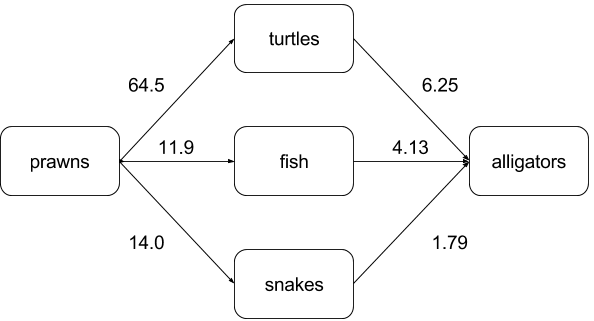
\includegraphics[width=.9\linewidth]{Ulano_ex.png}
\caption{Simplified network of carbon flows (in units of) 
in a southern Florida wetland. 
\textit{Source:~\cite{ulanowicz_quantifying_2009}}}
\label{fig:ulano_ex}
\end{figure}

To use ecological information metrics,  the network of flows are 
converted to an input-output
matrix format. The matrix contains a row and a column for each ``node,''
or species in the above ecosystem. In the $r$ x $c$ matrix $T$, 
cell $T_{ij}$
contains the volume of the flow from species \emph{i} to species \emph{j}.
For example, the above ecological network of flows could be
represented in the following input-output matrix:

\renewcommand{\kbldelim}{[}% Left delimiter
\renewcommand{\kbrdelim}{]}% Right delimiter

\begin{equation*}
T = 
\kbordermatrix{
   & p & t& f & s & a  \cr
 p & 0 & 64.5 & 11.9 & 14.0 & 0  \cr
 t & 0 & 0 & 0& 0& 6.25  \cr
 f &0 &0 & 0&0 &  4.13 \cr
 s &0 & 0& 0& 0 &  1.79 \cr
 a &0 & 0 & 0 & 0 & 0 \cr}
 \end{equation*}

The input-output model of inter-species flows
is based off the Leontief input-output matrix of
inter-industry flows for an economy.
Similar to an ecosystem, an economy consists of flows of
raw materials into industries, which transform
them into useful goods and services, which flow 
up the ``food chain'' to other industries
and ultimately to final users.
Economist Wassily Leontief won the Nobel memorial 
prize in Economics
for developing the input-output model 
of an economy. These ``I-O'' matrices are used extensively
by the U.S. Bureau of Economics Analysis (BEA)
and others to measure the output of industrial
sectors and the economy as a whole. I-O matrices
are also used to examine the inter-dependencies between 
industries. The I-O matrices can be used,
for example,
to forecast how a change in final demand will ripple 
backwards to affect employment levels in
all feeder industries. 

We come full circle then. Biology imported the I-O model 
from economics because of its usefulness to describe
ecosystem inter-species networks. We now explore
the usefulness of applying ecological
information metrics to summarize efficiency and
resiliency of the economy. The following section
uses the Florida wetland ecosystem example to illustrate
how it can be characterized  relative levels of efficiency and resiliency, an economy can be too.

\section{Describing Efficiency and Resiliency}
\cite{arthur_complexity_1999} and 
\citep{arthur_complexity_2015,colander_review_2002} and
many others have argued that the economy grows, or evolves,
like a complex adaptive system.~\citep{arthur_complexity_2015} 
If this is true, what metrics  
beyond GDP might be useful to evaluate the health of the
economy? One promising source is the work of 
Ulanowicz~\cite{ulanowicz_quantifying_2009}
based on the work of MacKay~\cite{}
and others who have applied measures of ecosystem vitality to
economic vitality. These measures arise from the
information, or network,  analysis of MacKay~\cite{}
and others. Recentlyl, King~\cite{} and Kharrazi~\cite{} have
applied these ecological information metrics to
the economy.

Ecologial information metrics can provide summary measures for networks 
of flows. An ecosystem can be seen as a network of flows of 
carbon, lower members of the food chain provide energy in 
the form of carbon (?)
to those who consume them. These flows of carbon can be
represented as an input-output matrix, similar to economic
Leontief I-O matrices. Ecological information metrics are 
a subset of information metrics that measure the vitality
of an ecosystem, where vitality includes both efficiency and
resiliency. 

Like an ecosystem, an economy's robustness is also a combination
of efficiency and resiliency. Efficiency is a reflection of
using the most efficient pathways (industries) to convert
raw materials into useful goods and services. This is 
often equated with maximizing output, or Gross Domestic Product (GDP).

However, also like an ecosystem, an economy must maintain
some redundancy, or less efficient pathways to allow
flexibility to unforeseen shocks. For example, suppose the most
efficient primary input into electricity coal, in the sense that the 
kiloJoules of energy from \$1 worth of coal is greater than other
possible primary inputs. The most efficient economy would
funnel all of its resources toward making electricity from coal.
However, should a shock to the coal supply arise, the economy
would crash and require a significant recovery time to 
invent new electricity production methods and develop
the appropriate infrastructure.

Thus, to be robust, an economy needs to build in
at least some redundancy along with efficiency. Redundancy
includes not only alternative ways to produce key goods and
services, but also innovation. For technology to evolve,
at least some human and physical capital must be diverted from
the production line to work in the research lab. This reduces
efficiency, but increases the overall robustness of the economy.

How might the robustness of an economy be measured? 


\section{Application to the U.S. Energy Sector}
Similar to this previous work, we will apply ecological
information metric to energy sectors of the economy using
Leontief Input-Output data publicly available from the U.S.
Bureau of Economic Analysis and the U.S. Energy
Information Administration.

%\end{multicols}
\subsection{Ecological Information Metrics}

\begin{table}[H]
\caption{Ecological Information Metrics.}
\label{IOmetrics}
\vskip 0.15in
\begin{center}
\begin{sc}
\begin{tabular}{ l l}
\hline

Metric &  Formula  \\
\hline
&  \\
Systemic Efficiency
  & $SE = \displaystyle\sum_{ij}{T_{ij}} log(\frac{T_{ij}TST}{T_{i.}T_{.j}}) $ 
  \\[.25in]

Reserve Capacity 
  & $RC = - \displaystyle\sum_{ij}{T_{ij}} log(\frac{T_{ij}^2}{T_{i.}T_{.j}}) $ 
 \\[.25in]
  
Capacity (SE + RC)
  & $C = -\displaystyle\sum_{ij}{T_{ij}} log(\frac{T_{ij}}{TST}) $ 
   \\[.25in]

Organized Power  & $\alpha=\frac{SE}{SE + RC}$  \\[.25in]

Fitness
 
 & $F = -[\frac{e}{log(e)}] 
    \alpha^\beta log(\alpha^\beta)$ \\[.25in]

& $F' = -e \beta \alpha^{\beta - 1}
\bigg(
    \frac{log(\alpha^\beta)}  {log(e)} 
        + 1 
\bigg)$         \\[.25in]

 


Robustness & $R = TST \cdot F$\\[.25in]


& $\frac{\partial R}{\partial T_{ij}} = F + \frac{TST \cdot F'}{C}
\bigg(log \big(\frac{T_{ij} \cdot TST}{T_{i.} T_{.j}} \big) 
+ \alpha log \big( \frac{T^{2}_{ij}}{T_{i.}T_{.j}} 
\big) \bigg)$ \\[.25in]





First-order Conditions & $F = 1, F'=0$ \\[.25in]




\end{tabular}
\end{sc}
\end{center}
\vskip -0.1in
\end{table}

where \\
\begin{tabular}{r l}
$T_{ij}$  & quantity that flows from sector $i$ to sector $j$ \\[.1in]
$T_{i.}$ & sum of all flows from sector $i$ \\
$T_{.j}$ & sum of all flows into sector $j$ \\
$TST$ & $1$x$1$ scalar containing Total System Throughput (i.e. $T_{..})$\\
$\mathbf{IO}$ & $r$ x $c$ IO matrix of flows \\
$\mathbf{R}$ &  $r$ x $1$ vector of row sums of the IO matrix\\
$\mathbf{C}$ &  $1$ x $c$ vector of column sums of the IO matrix \\
$\beta$ &  parameter to allow optimal $\alpha$ 
    to vary across contexts  \\
$\circ$ & element-wise multiplication of two equally-dimensioned
matrices\\
$log(\mathbf{M})$ & element-wise log transformation of the 
entries in matrix $\mathbf{M}$\\
$\frac{1}{\mathbf{M}}$ & element-wise inverse of the entries in 
matrix $\mathbf{M}$ \\
$\mathbf{M}^2$ & element-wise square transformation of the 
entries in matrix $\mathbf{M}$ \\
$GRAND \sum \mathbf{M}$ & sum of all entries 
in matrix $\mathbf{M}$ (e.g. $TST=GRAND\sum \mathbf{IO})$ \\


\end{tabular}


\medskip

\subsection{Interpretation}

  The constant, $-\frac{e}{log(e)}$, in the formula for \emph{Fitness} 
  is constructed so that the function on the value of 1 at the maximum. The adjustable parameter, $\beta$, 
  allows the optimal $alpha$ to vary across contexts. For example, 
  \cite{ulanowicz_quantifying_2009} suggests setting $\beta=1.288$ and 
  thus optimal $\alpha = .46$ for ecosystems. They estimated the 
  value based on observations of viable ecosystems and . By default, if $\beta=1$, then the Fitness function 
 is maximized at $\alpha = \frac{1}{e} = 0.3678$, an arbitrary choice.





\section*{Mathematical Appendix}
\begin{table}[H]
\caption{Matrix Formulation of Ecological Information Metrics.}
\label{IOmetrics_matrix}
\vskip 0.15in
\begin{sc}
\begin{center}
\begin{tabular}{ l l l }
\hline

Metric &  Formula & Matrix Formula \\
\hline
& & \\
%\hspace{.05in}
Systemic Efficiency
  & $SE = \displaystyle\sum_{ij}{T_{ij}}
  log(\frac{T_{ij}TST}{T_{i.}T_{.j}}) $ 
  & grand $\displaystyle\sum  \mathbf{IO} \circ 
  log\bigg(\mathbf{IO} \circ  \frac{TST}{\mathbf{R}\mathbf{C}}
  \bigg)$ \\[.25in]
  
  \multicolumn{3}{l}{\hspace{.5in} \texttt{mata code:
  SE=sum(IO:*(log(IO:*(TST:*(1:/(rowsum(IO)*colsum(IO)))))}} \\[.5in]

Reserve Capacity 
  & $RC = - \displaystyle\sum_{ij}{T_{ij}} log(\frac{T_{ij}^2}{T_{i.}T_{.j}}) $ 
  & -grand $\displaystyle\sum  \mathbf{IO} \circ 
  log\bigg(\mathbf{IO^2} \circ  \frac{1}{\mathbf{R} \mathbf{C}} \bigg)$ \\[.25in]
  
\multicolumn{3}{l}{\hspace{.5in} \texttt{mata code:
  RC=-sum(IO:*(log((IO:*IO):*(1:/(rowsum(IO)*colsum(IO)))))}} \\[.5in]
  
Capacity (SE + RC)
  & $C = -\displaystyle\sum_{ij}{T_{ij}} log(\frac{T_{ij}}{TST}) $ 
  & -grand $\displaystyle\sum  \mathbf{IO} \circ 
  log\bigg(\frac{1}{TST} \mathbf{IO}\bigg)$ \\[.25in]
  
\multicolumn{3}{l}{\hspace{.5in} \texttt{mata code:
  C=-sum(IO:*(log(IO:/TST)))}} \\[.5in]
  
\end{tabular}
\end{center}
\end{sc}
\vskip -0.1in
\end{table} 

\bibliographystyle{plainnat}
\bibliography{garden_economy}
\end{document} 


